%
% File acl2012.tex
%
% Contact: Maggie Li (cswjli@comp.polyu.edu.hk), Michael White (mwhite@ling.osu.edu)
%%
%% Based on the style files for ACL2008 by Joakim Nivre and Noah Smith
%% and that of ACL2010 by Jing-Shin Chang and Philipp Koehn


\documentclass[11pt,letterpaper]{article}
\usepackage[letterpaper]{geometry}
\usepackage{acl2012}
\usepackage{times}
\usepackage{latexsym}
\usepackage{amsmath}
\usepackage{amsfonts}
%\usepackage{cite}
% \usepackage[sort&compress]{natbib}
\usepackage{multirow}
\usepackage{graphicx}
\usepackage{url}
\graphicspath{ {images/} }
\makeatletter
\newcommand{\@BIBLABEL}{\@emptybiblabel}
\newcommand{\@emptybiblabel}[1]{}
\makeatother
\usepackage[hidelinks]{hyperref}
\DeclareMathOperator*{\argmax}{arg\,max}
\setlength\titlebox{6.5cm}    % Expanding the titlebox
\setlength{\thinmuskip}{0mu}
\setlength{\medmuskip}{0mu}
\setlength{\thickmuskip}{0mu} 

\title{Discrete Structured Representation Learning}

\author{Benjamin Striner \\
  {\tt bstriner@andrew.cmu.edu} \\}

\date{October 19, 2017}

\begin{document}
\maketitle
\begin{abstract}
Discrete structured representation learning allows the compression of information into a finite space and the representation of information in a manner that is understandable and explainable. Continuous neural networks are efficient to optimize but do not allow for easy interpretation. We present experiments optimizing over discrete hidden representations that can be interpreted as ontologies or decision trees. We also examine conventional post-mortem clustering and find that it frequently underperforms random assignments.
\end{abstract}

\section{Introduction}

Hidden representations inferred by neural networks are most frequently dense and continuous. Discrete representations are hard to interpret, so techniques for clustering, visualization, and dimensionality reduction are applied to make the hidden representation understandable. These analyses are typically applied to hidden representations ``post-mortem'' (after training).

Conventional linguistic ontologies attempt to organize words, concepts, or other objects into a discrete structure, typically a hierarchical tree (e.g., WordNet, PropBank). This type of representation tends to be more understandable than a dense matrix multiplication. Human knowledge is commonly and traditionally represented as facts, nodes, networks, or other types of discrete structures.

The ability to learn discrete representations allows for reduction in the number of bits required to encode each input \cite{Hu17}.
Structured discrete representations may have other advantages when used by higher-level models, such as better enabling logic and tree searching.

\section{Method}

We provide a method for expanding existing neural networks to learn a discrete hidden representation. To focus on the core optimization problems, we focus on one of the simplest models, learning a skipgram model as discussed in \cite{Mikolov1301} \cite{MikolovSCCD13}.

Let $X$ and $Y$ be two discrete variables. We will discuss methods for factoring the distribution $P(X,Y)$. Let the matrix $A$ represent the joint distribution.

$$A_{x,y}=P(X=x, Y=y)$$

The entropy of the marginal distribution, $H(Y)$, measures the complexity of the data if only $Y$ is considered. In the case of a skipgram matrix, this is roughly the entropy of the unigram distribution.

\begin{align*}
h(x) &= -x \log(x) \\
P(Y=y) &= \sum_x P(X=x, Y=y) \\
H(Y) &=  \sum_y h(P(Y=y))
\end{align*}

The conditional entropy, $H(Y \mid X)$, measures the complexity of $Y$ if $X$ is known. A neural network trained given $X$ to predict $Y$ using cross-entropy loss will at best achieve this value. The conditional entropy is the joint probability times the log of the conditional probability, or alternatively the marginal probability times the entropy of the conditional distribution.

$$H(Y \mid X)=-\sum_{x,y} P(X, Y) \log(P(Y \mid X)) $$
$$P(X,Y) = P(X) P(Y \mid X)$$
$$H(Y \mid X)= \sum_{x,y}  P(X) h(P(Y \mid X))$$

The function $f(x)=-x \log(x)$ is concave. The entropy of a linear combination of distributions is greater than or equal to the linear combination of the entropy of the distributions. The entropy of the marginal distribution is greater than or equal to the conditional entropy.

\subsection{Continuous factoring}

A common method of continuous factoring is to embed each input into a continuous representation. A neural network is used to parameterize an approximation ($\tilde{P}$) to the actual conditional distribution. The loss ($J$) is the expected negative log conditional likelihood. See, for example, \cite{MikolovSCCD13} and \cite{Mikolov1301}. 

A simple version of this model is parameterized by embeddings ($U$), weights ($W$) and bias ($b$) and uses a softmax to squash the outputs.

$$ \tilde{P}(Y\mid X) = \operatorname{softmax}(U W+b)$$
$$ J = -\sum_{x, y} P(Y,X) \log \tilde{P}(Y \mid X) $$
$$ J = -\mathbb{E}_{[x,y \sim X, Y]} \log \tilde{P}(Y \mid X) $$

\subsection{Discrete factoring or clustering}

A common practice for producing discrete clusters is to train a neural network and then apply clustering techniques (e.g., GMM, K-means) to the learned continuous hidden space. We examine how much information is actually retained by applying clustering to learned embeddings. We also examine methods to directly cluster with respect to a given loss function.

If examples in a dataset are clustered, the single output that minimizes the loss for a given cluster may be calculated analytically or iteratively. In the case of minimizing entropy, constrained by the space of valid distributions, the analytic solution is straightforward.

$$\min_{\tilde{x}}[\sum_i-x_i \log(\tilde{x_i})] = x$$

The expected negative log conditional likelihood is the conditional entropy of the combined distributions, analogous to the cross entropy loss in above discussion of continuous factoring. Similar approaches could be applied to more complicated neural networks, but discrete factorization of a conditional distribution is highly efficient and works well for analysis of the core optimization problem.

Let $X$ be clustered into a discrete space $Z$. Let $C$ be an indicator matrix where $C_{z,x}$ indicates that $X=x$ is a member of $Z=z$. $C$ encodes the distribution $P(Z \mid X)$. $C$ is constrained to all $0$ except one and only one $1$ per column. The joint distribution matrix $B_{i,j}=P(Y=j,Z=i)$ is efficiently calculated using the dot product. Note that $Z$ and $Y$ are independent given $X$.

$$P(Z \mid X,Y) = P(Z \mid X)$$
$$P(Y,Z) = \sum_x P(Y,X) P(Z \mid X)$$
$$B = C A $$ 

If the inputs $X$ are encoded discretely into $Z$ where $Z$ is overfull, some information is lost.  The matrix $B$, $P(Y,Z)$, is a linear combination of rows of the matrix $A$, $P(Y,X)$. Therefore $H(Y \mid Z) \ge H(Y \mid X)$. 

By relaxing the constraints on $C$, we can create a parameterization of $P(Z \mid X)$ that allows for gradient descent on the conditional entropy $H(Y\mid Z)$. A simple parameterization
is $C=\operatorname{softmax}(W)$. If the softmax is fully saturated, each input, $X$, will be assigned to one and only one cluster, $Z$. At initialization, each row is assigned to a random mixture of clusters. The softmax ensures that $C$ may be vallidly interpreted as $P(Z \mid X)$. By the concavity of $h$, we predict that the model will tend towards saturation. A mixture of distributions will have a higher entropy than the component distributions.

$$ J = H(Y \mid X) $$
$$ J = - \sum_{y,z} P(Y, Z) \log( P(Y \mid Z)) $$

For more complicated relationships, it may become necessary to approximate $P(Y \mid Z)$ with a neural network as well. In that case the following formulation may be the most useful. The two parameterized values are $\tilde{P}(Y \mid Z)$ and $P(Z \mid X)$.

$$ J = - \sum_{y,z,x} P(Y, Z) P(Z \mid X) \log( \tilde{P}(Y \mid Z)) $$
$$ J = - \mathbb{E}_{x,y \sim X, Y} \sum_{z} P(Z \mid X) \log( \tilde{P}(Y \mid Z)) $$

\subsection{Hierarchical clustering}

The simplest discrete structured encoding is a binary tree. The address of a node in a binary tree of depth $d$ may be represented as a vector of length $d$ containing only zeros and ones. A complete binary tree will contain $2^d$ leaves at the base of the tree and will ideally achieve similar performance to models using $2^d$ flat clusters.

A reasonable loss for hierarchical clusters is the weighted sum of the conditional entropy of the clusters at each depth in the tree. In the spirit of the Bellman equation, an exponential series is a reasonable choice of weighting. Let $Z_d$ be the address of $X$ in the tree starting with $Z_0$ at the root.

$$ J = \sum_d \beta ^ d  H(Y \mid Z_0,\ldots, Z_d) $$

Intuitively, one is optimizing a weighted sum of how much information is available given the depth ($d$) of the tree or how many bits of the representation are provided. The parameter $\beta$ controls the balance of having more information available early or better accuracy given more of the tree. This model attempts to pack more information into the early bits and remaining differentiation into the later bits. The meaning of the later bits is dependent on the earlier bits but the converse is not true.

We parameterize clusters at at the bottom layer of the tree $C_d$. We calculate the membership of clusters at previous layers $C_0,...,C_{d-1}$ by summing leaves into parent nodes. We calculate the weighted loss over tree depth as described above.

\subsection{Regularization}

We experimented with several forms of regularization to examine the effects of regularization choice and weight on the performance of each model.

$L_1$ regularization penalizes the sum of the absolute values of the weights.

$$L_1(W) = \sum_{i,j} \lvert W_{i,j} \rvert $$

$L_2$ regularization penalizes the sum of the squares of the weights.

$$L_2(W) = \sum_{i,j} (W_{i,j})^2 $$

The exclusive lasso regularizer models the scenario when variables in the same group compete with each other and has been proven successful for inducing sparsity
\cite{zhou10a}, 
\cite{bach2012},
 \cite{Campbell15}.

$$V(W) = \sum_i (\sum_j \lvert W_{i,j} \rvert)^2$$ 

We also experimented with activity regularization. We want to ensure that the model fully utilizes all of the available clusters, so would like a regularizer that prevents the marginal probability of any cluster from going to zero. We chose a logistic barrier regularizer applied to the marginal cluster probability. This regularizer approaches infinity as the expexted probability of any cluster approaches zero.

$$ R(P) = -\sum_z \log[ \mathbb{E}_{x \sim \operatorname{unif}(X)} P(Z=z \mid X=x)]$$ 

We performed experiments using $\mathbb{E}_{x \sim X}$, $R_0(P)=\sum_z \log P(Z)$ but this performed poorly in comparison to the expectation drawing from a uniform distribution.

$$R_0(P) =  -\sum_z \log [ \mathbb{E}_{x \sim X} P(Z=z \mid X=x) ]$$ 
$$R_0(P) =  -\sum_z \log P(Z=z )$$ 

\section{Experiments and Results}

We built a skipgram matrix from the Brown corpus as a simple distribution so we could focus on aspects of the optimization problem. We removed all non-alphabetic characters and capitalization. We replaced all words that appeared less than 20 times with an unknown symbol, resulting in a set of $n=4,946$ symbols (including the unknown symbol). We then enumerated all words within a $k$ word window around each word to produce a list of skipgrams ($k$=3). We calculated the joint distribution by tabulating these skipgrams into a $n$ by $n$ matrix.

The entropy of the marginal distribution created from our matrix is 5.913 and the conditional entropy of the matrix is 5.326. Any reasonable factorization of the matrix should result in performance somewhere between those two values.

\subsection{Random clustering}

We assessed an initial baseline by randomly and uniformly assigning words to clusters. As expected, as the number of clusters increased, the conditional entropy of the output given the cluster decreased (Figure \ref{f:random}). Given two clusters, the mean conditional entropy is 5.9109 ($\sigma=0.0004$). Given 1024 clusters, the mean conditional entropy is 5.5664 ($\sigma=0.0018$).

\begin{figure}
  \caption{Random uniform clustering}
\label{f:random}
  \centering
    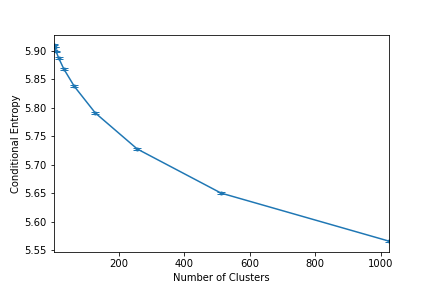
\includegraphics[width=0.5\textwidth]{random.png}
\end{figure}

\subsection{Skipgram models}

We trained unregularized continuous skipgram models varying the number of hidden units and found that performance asymptotically approached the analytically calculated conditional entropy (Figure \ref{f:baseline}). 

\begin{figure}
  \caption{Continuous skipgram model}
\label{f:baseline}
  \centering
    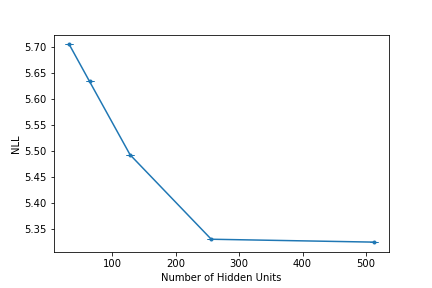
\includegraphics[width=0.5\textwidth]{baseline.png}
\end{figure}

We additionally trained models with $L_1$ and $L_2$ regularization. We used these models to examine how regularization and the number of hidden units affect the quality of post-mortem clustering. 

\subsection{Vocabulary clustering ($k=2$)}

We trained our model to discretely factor the matrix into 2 clusters of words. The mean conditional entropy of the resulting matrix was 5.8856 ($\sigma=4.4e-08$). This outperforms both the random baseline and any iteration of post-mortem clustering. Additionally, the standard deviation of this model is roughly five orders of magnitude below most of the post-mortem clusterings.

We clustered the hidden representations learned by each of our continuous skipgram models into 1024 groups using GMM clustering (Figure \ref{f:bgmm}) and k-means clustering (Figure \ref{f:km}). The best performance of any post-mortem binary clustering trial was 5.89231. Many trials performed at or worse than random. GMM only performed better than random when a large number of hidden units were used. KMeans clustering performed better than random and GMM when a small number of hidden units were used.

\begin{figure}
  \caption{Binary GMM clustering}
\label{f:bgmm}
  \centering
    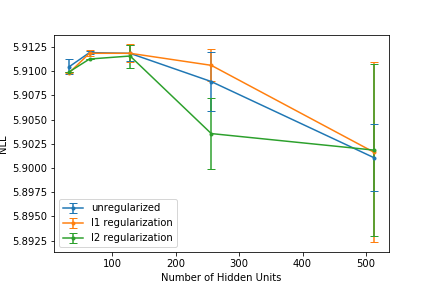
\includegraphics[width=0.5\textwidth]{binary_gmm.png}
\end{figure}

\begin{figure}
  \caption{Binary K-means clustering}
\label{f:bkm}
  \centering
    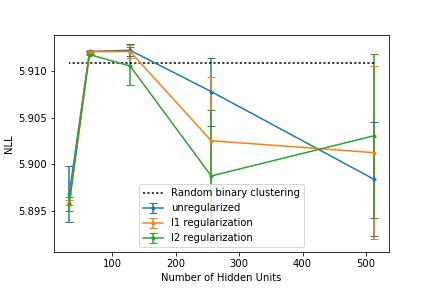
\includegraphics[width=0.5\textwidth]{binary_km.png}
\end{figure}

\subsection{Vocabulary clustering ($k=1024$)}

We trained our model to cluster the vocabulary into 1024 groups. The mean conditional entropy of the resulting clusters was 5.5480 ($\sigma=0.00078$), outperforming random clustering and post-mortem clustering. The model accomplished this performance without utilizing all clusters, so we knew that improvements were possible. The average utilization (out of 1024 clusters) was 809.4 ($\sigma=4.8$). We experimented with using regularization to increase the average utilization.

We trained models with varying regularizer weights to determine the effect regularizer choice and weight has on conditional entropy and utilization. We experimented with the discussed barrier (Figure \ref{f:fb}), exclusive lasso (Figure \ref{f:fel}), $L_1$ (Figure \ref{f:fl1}), and $L_2$ (Figure \ref{f:fl2}) regularizers. The barrier and exclusive lasso regularizers achieve similar performance, 5.5175 and 5.5166 respectively. The L1 regularizer was effective at increasing utilization but caused poor clustering. The L2 regularizer causes decreased clustering performance.

\begin{figure}
  \caption{Uniform Prior Regularization ($k=1024$)}
\label{f:fb}
  \centering
    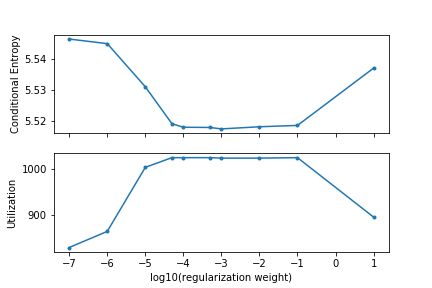
\includegraphics[width=0.5\textwidth]{skipgram_flat_b.png}
\end{figure}
\begin{figure}
  \caption{Exclusive Lasso Regularization ($k=1024$)}
\label{f:fel}
  \centering
    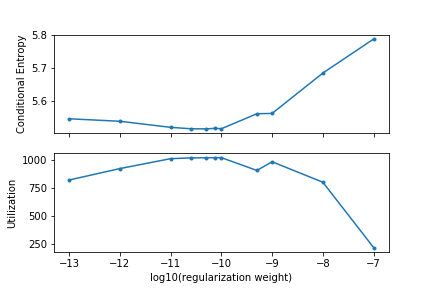
\includegraphics[width=0.5\textwidth]{skipgram_flat_el.png}
\end{figure}
\begin{figure}
  \caption{L1 Regularization ($k=1024$)}
\label{f:fl1}
  \centering
    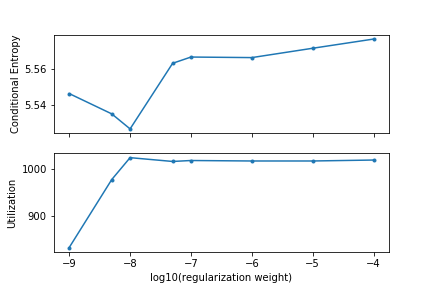
\includegraphics[width=0.5\textwidth]{skipgram_flat_l1.png}
\end{figure}
\begin{figure}
  \caption{L2 Regularization ($k=1024$)}
\label{f:fl2}
  \centering
    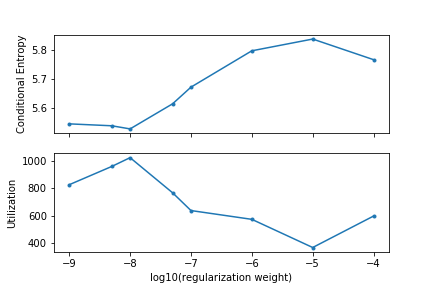
\includegraphics[width=0.5\textwidth]{skipgram_flat_l2.png}
\end{figure}

We clustered the hidden representations learned by each of our continuous skipgram models into 1024 groups using GMM clustering (Figure \ref{f:fgmm}) and k-means clustering (Figure \ref{f:fkm}). The best performance of any post-mortem clustering with $k=1024$ was 5.59504.

Both GMM and $k$-means show clearer trends with $k=1024$ than $k=2$. Without regularization, small numbers of hidden dimensions cluster better than large numbers of hidden dimensions. With regularization, small and large numbers of hidden dimensions cluster better than a medium number of hidden dimensions.

\begin{figure}
  \caption{GMM clustering ($k=1024$)}
\label{f:fgmm}
  \centering
    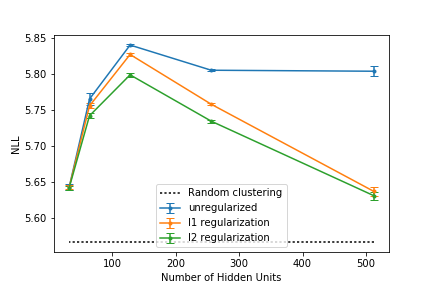
\includegraphics[width=0.5\textwidth]{flat_gmm.png}
\end{figure}


\begin{figure}
  \caption{K-means clustering ($k=1024$)}
\label{f:fkm}
  \centering
    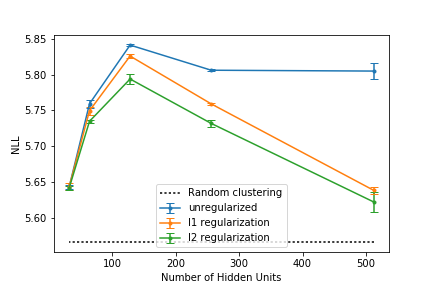
\includegraphics[width=0.5\textwidth]{flat_km.png}
\end{figure}

\subsection{Binary tree clustering}

We trained binary trees of depth 10 so as to compare to our flat models of 1024 ($2^{10}$) clusters.

We trained our binary tree model varying $\beta$ to analyze the effect of the Bellman decay parameter (Figure \ref{f:beta}). Increasiing $\beta$ produces better performance at deeper levels of the tree but worse performance near the root of the tree, and vice versa.

\begin{figure}
  \caption{Effect of Beta Hyperparameter}
\label{f:beta}
  \centering
    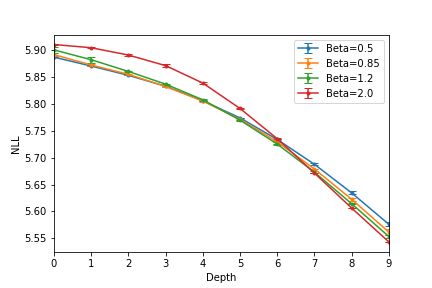
\includegraphics[width=0.5\textwidth]{skipgram_tree.png}
\end{figure}

Adding regularization to our binary tree model improved performance at the bottom of the tree while only slighlty impacting performance at the top of the tree. For example, see Figure \ref{f:btb} and \ref{f:btel} for the effect of barrier and exclusive lasso regularization weight given $\beta=0.85$. It is impossible to identify a single ``best'' model, as the choice of $\beta$ depends on application.

\begin{figure}
  \caption{Binary tree with barrier regularizer ($\beta=0.85$)}
\label{f:btb}
  \centering
    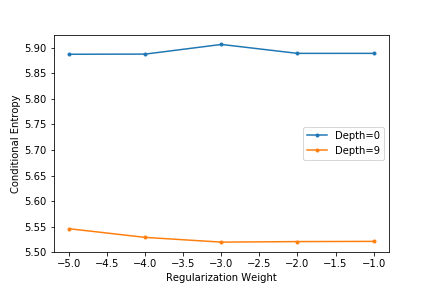
\includegraphics[width=0.5\textwidth]{skipgram_tree_b_0.png}
\end{figure}
\begin{figure}
  \caption{Binary tree with exclusive lasso regularizer ($\beta=0.85$)}
\label{f:btel}
  \centering
    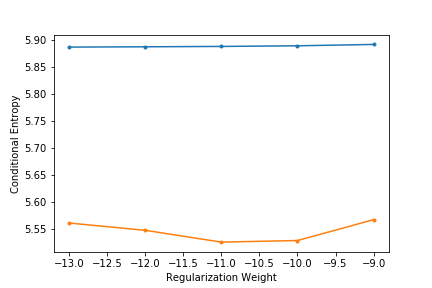
\includegraphics[width=0.5\textwidth]{skipgram_tree_el_0.png}
\end{figure}

\section{Discussion}

Optimizing the conditional entropy of $P(Y\mid Z)$ was an effective method of forming clusters. Clusters contained more information regarding $Y$ than clusters created using post-mortem methods.

Although clustering hidden representations should intuitively capture information related to the objective, we found that this was frequently not the case. In many situations, post-mortem clustering of hidden representations produced worse clusters than random clustering. Regularization and the size of the hidden space have strong effects on the result of the clustering, which can be avoided by using our proposed models.

Regularization prevented underutilization caused by death of some clusters. Barrier and exclusive lasso regularizers prevented underutilization. It is critical to fully understand the dynamics of the optimization problem in such a simple environment, so it can be applied to more complicated networks.

\section{Conclustion}
Discrete structured representations are natural and understandable. There are many challenges involved in learning discrete representations of a given model, above and beyond the challenges of the model itself. Learning a knowledge representation comparabile to a traditional semantic ontology like WordNet or PropBank requires both datasets and models for extracting semantic content, and a data structure capable of representing an ontology. 

These experiments address the simplest possible ontology, a binary tree. Even such a simple model can be interpreted as a decision tree, and is more explainable and understandable than a dense calculation. Further systems for discrete optimization should enable a higher class of structures, potentially able to represent discrete logic.

\bibliography{tacl}
\bibliographystyle{acl2012}


\end{document}



